\documentclass{ctexart}

\usepackage{hyperref}
\usepackage{listings}
\usepackage{color}
\usepackage{xcolor}

\usepackage{tikz}
\usetikzlibrary{arrows,shapes,snakes,automata,backgrounds,petri,matrix}

\title{嵌入式操作系统实验报告}
\author{李约瀚 \\ 14130140331}

\definecolor{t1C}{rgb}{0,1,0}
\definecolor{t2C}{rgb}{1,0,0}
\definecolor{initC}{rgb}{0,0,1}


\lstset{tabsize=4,
    language=c,
    frame=shadowbox,
    commentstyle=\color{red!50!green!50!blue!50},
    rulesepcolor=\color{red!20!green!20!blue!20},
    keywordstyle=\color{blue!90}\bfseries, 
    showstringspaces=false,
    stringstyle=\ttfamily,
    keepspaces=true,
    breakindent=22pt,
    numbers=left,
    stepnumber=1,
    numberstyle=\tiny,
    basicstyle=\footnotesize,
    showspaces=false,
    flexiblecolumns=true,
    breaklines=true,
    breakautoindent=true,
    breakindent=4em,
    aboveskip=1em,
    fontadjust,
    captionpos=t,
    framextopmargin=2pt,framexbottommargin=2pt,abovecaptionskip=-3pt,
    belowcaptionskip=3pt,
    xleftmargin=3em,xrightmargin=3em,
    texcl=true,
}

\begin{document}
    \maketitle
    \newpage
    \tableofcontents
    \newpage
    
    \section{uCOS-II 的移植}
    \label{sec:ucosii-transplate}
    
    实验室使用的是 STM32F103ZET 的开发版一块。并使用基于 crosstool-ng 自行构建的 GNU-GCC
    交叉编译工具链。
    
    \subsection{交叉编译工具链构建}
    \label{sec:ucosii-transplate:crosstool-chain}
    
    本次实验使用 \href{http://crosstool-ng.github.io/}{crosstool-NG}-1.23 构建。直接基于
    预设的 arm 架构无系统配置。
    \begin{lstlisting}
    ct-ng arm-unknown-eabi
    ct-ng build
    \end{lstlisting}
    然后可获得交叉编译至 无操作系统的 arm 架构平台。
    
    其中由于 STM32F03ZET6 是基于 arm 的 cortex-m3 架构,同时不需要使用 C 标准库。
    故在编译标志中需要添加
    \begin{lstlisting}
    -mcpu=cortex-m3 -mthumb -nostdlib
    \end{lstlisting}
    
    \subsection{CMake 与 STM32F1x 固件库配置}
    \label{sec:ucosii-transplate:cmakeNstm32f1x}
    
    \lstinline|CMakeList.txt| 参照 cmake 官方教程编写即可。
    其中需要将 cmake 中系统相关的内容设置为 \verb|Gerneric| 和 \verb|arm|。
    然后整个项目的语言是包括 \verb|C| 和 \verb|ASM|。
    
    配置 GNU-C 编译器为 \lstinline|${ARM_PREFIX}gcc}|, 同时 GNU-C++ 编译器配置为 
    \lstinline|${ARM_PREFIX}g++}|\footnote{本次试验为使用到C++编译器。}。
    此外按照 STM32F1x 固件库中的要求定义适合于 STM32F103ZET 的宏 \lstinline|STM32F10X_HD|。
    
    之后配置 include 目录,和连接静态库的目录\footnote{这里使用到了一个是MCU的固件库,还有一个是自己写的提供了
    \lstinline|printk| 输出函数的库。}
    
    最后配置连接器的参数,因为要初始化设备内存相关的和入口函数,需要手工编写一个连接器配置脚本。
    
    \subsection{uCOS-II 移植}
    \label{sec:ucosii-transplate:tp}
    
    官方已经有移植好的,选择基于 GNU 工具链的版本\footnote{非 GNU 工具链版本使用的是 Intel 风格的汇编
    GNU 的 GCC 编译器是 AT\&T 风格的。}。
    其中移植的过程相对简单主要是包括如下内容:
    \begin{itemize}
        \item 编写简单的 Bootloader,修改自 ST 官方固件库中的例程。
        \item 修改入口函数
        \item 修改中断向量表
    \end{itemize}

    \paragraph{Bootloader}
    直接复制 ST 官方标准的 Bootloader 即可。 需要注意官方的例程的入口函数是 \lstinline|Reset_System|,
    需要和连接器的脚本对应\footnote{官方的连接器脚本例程中是对应的。}。
    
    \paragraph{入口函数}
    在 注释\lstinline[language=C]|/* Call the application's entry point.*/|下面
    是跳转到 实际的入口函数,这个按照一般方式设置成 \lstinline|main| 函数。
    此外 ST 官方的固件库提供了 \lstinline|SystemInit| 函数用来初始化底层硬件,例如处理器的倍频。
    在无条件跳转 到main函数之前,应该先调用 \lstinline|SystemInit| 初始化硬件。
    
    \paragraph{中断向量表}
    在 Bootloader 中修改中断向量有关的,并将 \verb|PendSV| 中断和 \verb|SysTick| 中断对应的
    处理函数分别设置成 uCOS 提供的两个函数 \lstinline|OS_CPU_PendSVHandler| 和 \lstinline|OS_CPU_SysTickHandler|。
    
    \subsection{其他}
    \label{sec:ucosii-transplate:more}
     
    实验代码和移植代码可以分别在 \href{https://github.com/Qinka/uCOS-exp}{uCOS-exp},
    \href{https://github.com/Qinka/ucos-ii-stm32f103ze}{ucos-ii-stm32f103ze},和
    \href{https://github.com/Qinka/libaikit/tree/0.1/dev/master}{libaikit}找到。
        
    此外实验还使用到 OpenOCD 与 GDB 最为调试工具。
    
    \section{任务的基本管理}
    \label{sec:task-mang}
    
    \subsection{实验目的}
    
    \begin{enumerate}
        \item 理解任务管理的基本原理,了解任务的各个基本状态及其变迁过程;
        \item 掌握µC/OS-II中任务管理的基本方法(创建、启动、挂起、解挂任务);
        \item 熟练使用µC/OS-II任务管理的基本系统调用。
    \end{enumerate}
    
    \subsection{实验原理及程序结构}
    
    \subsubsection{实验设计}
    
    为了展现任务的各种基本状态及其变迁过程,本实验设计了Task0、Task1两个任务:任务Task0不断地挂起自己,再被任务Task1解挂,两个任务不断地切换执行。通过本实验,读者可以清晰地了解到任务在各个时刻的状态以及状态变迁的原因。
   
    
    \begin{figure}
        \centering
        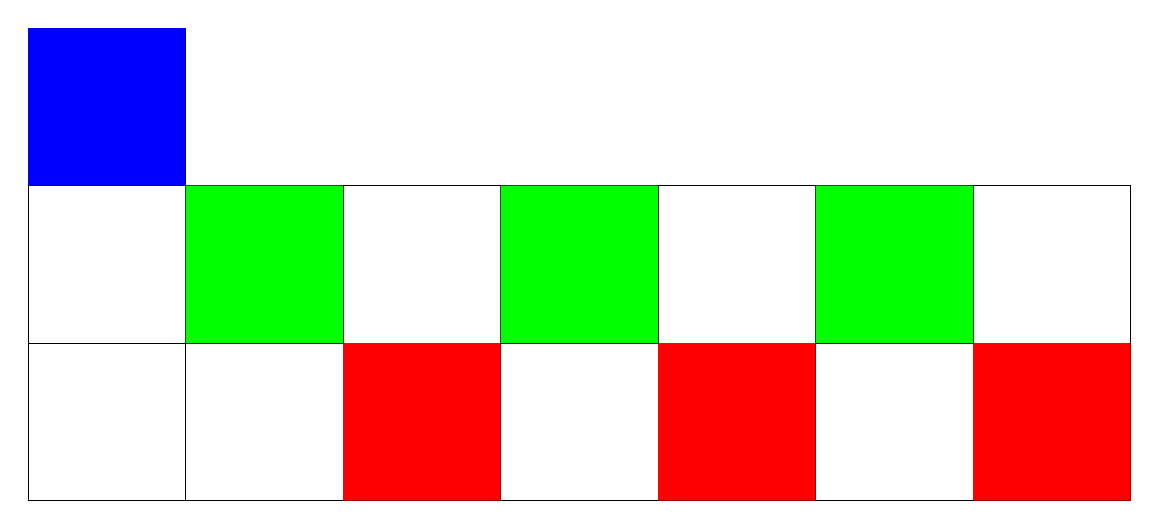
\begin{tikzpicture}
        \newcommand\fillGrid[2]{\fill[fill=#1,shift={#2}] (0,0) -- (0,2) -- (2,2) -- (2,0) --(0,0)}
        \draw[step=2cm](0,0) grid (14,4);
        \draw[step=2cm](0,4) grid (2,6);
        \fillGrid{initC}{(0,4)};
        \fillGrid{t1C}{(2,2)};
        \fillGrid{t2C}{(4,0)};
        \fillGrid{t1C}{(6,2)};
        \fillGrid{t2C}{(8,0)};
        \fillGrid{t1C}{(10,2)};
        \fillGrid{t2C}{(12,0)};
        \end{tikzpicture}
        \caption{任务先后关系。{\color{initC}蓝色}方格代表初始化任务,{\color{t1C}绿色}是 \textit{任务一},
            {\color{t2C}红色}是 \textit{任务二}}
        \label{fig:tm-1}
    \end{figure}
    
    \subsubsection{运行流程}
    整个应用的运行流程如图\ref{fig:tm-1}所示,其描述如下:
    \begin{enumerate}
        \item 系统经历一系列的初始化过程后进入 \lstinline|boot_card()| 函数,
            在其中调用\lstinline|ucBsp_init()|进行板级初始化后,调用 \lstinline|main()| 函数。
        \item \lstinline|main()| 函数调用 \lstinline|OSInit()|函数对µC/OS-II内核进行初始化,
            调用\lstinline|OSTaskCreate()| 创建起始任务 \verb|TaskStart|。
        \item \lstinline|main()| 函数调用函数 \lstinline|OSStart()| 启动µC/OS-II内核的运行,
            开始多任务的调度, 执行当前优先级最高的就绪任务 \verb|TaskStart|。
        \item \verb|TaskStart| 完成如下工作:
            \begin{enumerate}
                \item 安装时钟中断并初始化时钟,创建2个应用任务;
                \item 挂起自己(不再被其它任务唤醒),系统切换到当前优先级最高的就绪任务 \verb|Task0|。
            \end{enumerate}
    \end{enumerate}

    之后整个系统的运行流程如下:
    \begin{itemize}
        \item $t_1$ 时刻,Task0开始执行,它运行到$t_2$时刻挂起自己
        \item $t_2$ 时刻,系统调度处于就绪状态的优先级最高任务Task1执行
        \item $t_3$ 时刻,Task1唤醒Task0,后者由于优先级较高而抢占CPU
        \item $t_4$ 时刻,Task0又挂起自己,内核调度Task1执行
        \item $t_5$ 时刻,Task1再度唤醒Task0
    \end{itemize}
    \subsubsection{源程序说明}
    系统启动后,经历一系列的初始化过程,进入 \lstinline|main()| 函数,这是我们编写实现应用程序的起点。
    首先需要在 \lstinline|main()| 函数里创建起始任务 \verb|TaskStart|:
    \begin{lstlisting}
OSTaskCreate(TaskStart, (void *)0, &TaskStartStk[TASK_STK_SIZE - 1], 4);
    \end{lstlisting}
    
    \paragraph{TaskStart 任务}
    TaskStart 负责创建系统任务。
    \begin{lstlisting}
void  TaskStart (void *pdata) {
    // Allocate storage for CPU status register
    OS_CPU_SR  cpu_sr;
    // Create all the application tasks
    TaskStartCreateTasks();
    // Suspend the TaskStart
    OSTaskSuspend(OS_PRIO_SELF);
}
    \end{lstlisting}
    具体负责应用任务创建的 \lstinline|TaskStartCreateTasks()| 函数代码如下,
    它创建了两个应用任务 \verb|Task0| 和 \verb|Task1|
    \begin{lstlisting}
void  TaskStartCreateTasks (void) {
    INT8U  i;
    for (i = 0; i < N_TASKS; i++) // Create tasks
    // Each task will display its own information
        TaskData[i] =  i;
    OSTaskCreate(Task0, (void *)&TaskData[0], &TaskStk[0][TASK_STK_SIZE - 1], 5);
    OSTaskCreate(Task1, (void *)&TaskData[1], &TaskStk[1][TASK_STK_SIZE - 1], 6);
}
    \end{lstlisting}
    
    \paragraph{应用任务}
    应用任务 \verb|Task0|运行后将自己挂起,之后操作系统就会调度处于就绪状态的优先级最高的任务,具体代码如下。
    \begin{lstlisting}
void  Task0 (void *pdata) {
    INT8U i;
    INT8U err;
    i=*(int *)pdata;
    while(1) {
        // light LED
        LEDR_ON;
        kprint("");
        kprint("The application tasks switch counts: 0x%u",++count);
        kprint("Task0 is   running.");
        kprint("Task1 is   suspended.");
        kprint("");
        // light LEDc
        LEDR_OFF;
        // suspend itself 
        err=OSTaskSuspend(5);
    }
}
    \end{lstlisting}
    应用任务 \verb|Task1| 运行后将 \verb|Task0| 唤醒,使其进入到就绪队列中。
    \begin{lstlisting}
void  Task1 (void *pdata) {
    INT8U i;
    INT8U err;
    i=*(int *)pdata;
    while(1) {
        // change led
        LED1_ON;
        LED2_OFF;
        OSTimeDly(150);
        kprint("");
        kprint("The application tasks switch counts: 0x%u",++count);
        kprint("Task0 is   suspended.");
        kprint("Task1 is   running.");
        kprint("");
        OSTimeDly(150);
        // change led
        LED1_OFF;
        LED2_ON;
        // resume task0 
        err=OSTaskResume(5);
    }
}
    \end{lstlisting}
    
    \subsection{运行结果}
    
    在 使用工具链编译并使用 OpenOCD 搭配 STLinkv2 烧写并调试程序。
    然后 系统内核会依次调度两个任务。并得到如下输出。
    \begin{lstlisting}[language={}]
0000000000000000: Ucos-II loaded
0400000000000000:
0600000000000000:
0800000000000000: The application tasks switch counts: 0x01000000
0F00000000000000: Task0 is   running.
1400000000000000: Task1 is   suspended.
1800000000000000:
2D00000000000000:
2F00000000000000: The application tasks switch counts: 0x02000000
3600000000000000: Task0 is   suspended.
3B00000000000000: Task1 is   running.
3F00000000000000:
5300000000000000:
5500000000000000: The application tasks switch counts: 0x03000000
5C00000000000000: Task0 is   running.
6100000000000000: Task1 is   suspended.
6500000000000000:
7900000000000000:
7C00000000000000: The application tasks switch counts: 0x04000000
8300000000000000: Task0 is   suspended.
8700000000000000: Task1 is   running.
8C00000000000000:
    \end{lstlisting}
    \subsection{实验细节}
    
    在 \verb|Task0| 与 \verb|Task1| 交替执行的时候,系统中还包含 空闲任务。空闲任务在系统初始化的时候初始化的。
    
    \section{优先级反转}
    
    \subsection{实验目的}
    掌握在基于优先级的可抢占嵌入式实时操作系统的应用中,出现优先级反转现象的原理。
    
    \subsection{原理及程序结构}
    
    \subsubsection{实验设计}
    
    \paragraph{优先级反转原理}
    
    在本实验中,要体现嵌入式实时内核的优先级抢占调度的策略,并显现由于共享资源的互斥访问而出现的优先级反转现象。
    
    优先级反转发生在有多个任务需要使用共享资源的情况下,可能会出现高优先级任务被低优先级任务阻塞,
    并等待低优先级任务执行的现象。高优先级任务需要等待低优先级任务释放资源,而低优先级任务又正在等待中等优先级任务,
    这种现象就被称为优先级反转。两个任务都试图访问共享资源是出现优先级反转最通常的情况。
    为了保证一致性,这种访问应该是顺序进行的。如果高优先级任务首先访问共享资源,则会保持共享资源访问的合适的任务优先级顺序;
    但如果是低优先级任务首先获得共享资源的访问,然后高优先级任务请求对共享资源的访问,则高优先级任务被阻塞,
    直到低优先级任务完成对共享资源的访问。
    
    \paragraph{设计要点}
    
    \begin{enumerate}
        \item 设计了3个应用任务TA0~TA2,其优先级逐渐降低,任务TA0的优先级最高。
        \item 除任务TA1外,其它应用任务都要使用同一种资源,该资源必须被互斥使用。
            为此,创建一个二值信号量mutex来模拟该资源。虽然μC/OS-Ⅱ在创建信号量时可以选择采用防止优先级反转的策略,
            但在本实验中我们不使用这种策略。
        \item 应用任务的执行情况如图\ref{fig:pt-1}所示
    \end{enumerate}
    \begin{figure}
        \centering
        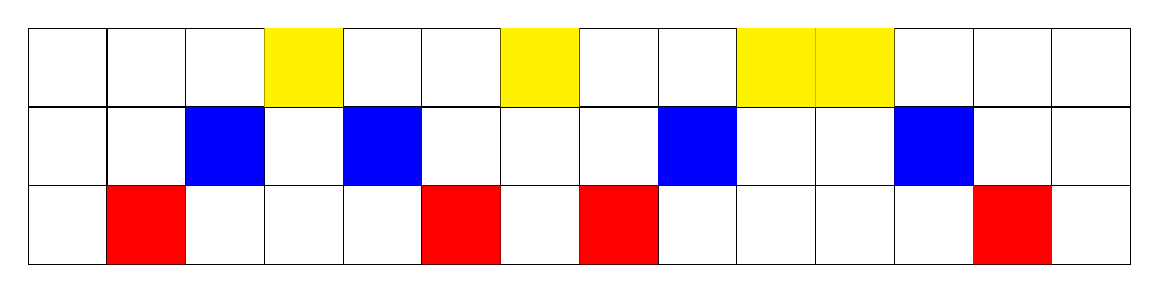
\begin{tikzpicture}
        \newcommand\fillGrid[2]{\fill[fill=#1,shift={#2}] (0,0) -- (0,1) -- (1,1) -- (1,0) --(0,0)}
        \draw[step=1cm](0,0) grid (14,3);
        \fillGrid{red}{(1,0)};
        \fillGrid{blue}{(2,1)};
        \fillGrid{yellow}{(3,2)};
        \fillGrid{blue}{(4,1)};
        \fillGrid{red}{(5,0)};
        \fillGrid{yellow}{(6,2)};
        \fillGrid{blue}{(11,1)};
        \fillGrid{red}{(7,0)};
        \fillGrid{blue}{(8,1)};
        \fillGrid{yellow}{(9,2)};
        \fillGrid{yellow}{(10,2)};
        \fillGrid{red}{(12,0)};
        \end{tikzpicture}
        \caption{任务先后关系。{\color{blue}蓝色}方格代表\textit{任务一},
            {\color{yellow}黄色}是 \textit{任务零},
            {\color{t2C}红色}是 \textit{任务二}}
        \label{fig:pt-1}
    \end{figure}

    \subsubsection{系统的运行流程}
    
    \begin{enumerate}
        \item 系统初始化,之后进入main函数;
        \item 在main函数中,首先创建一个二值的信号量mutex;
        \item  在main函数中创建TaskStart任务,由TaskStart任务创建所有的应用任务(TA0、TA1、TA2)。优先级较高的任务TA0、TA1先延时若干个时钟节拍,以便低优先级任务TA2运行。
        \item $t_1$时刻,任务TA2运行并首先申请到信号量mutex;
        \item $t_2$时刻,任务TA1延时到期,任务TA1的优先级高于任务TA2的优先级,因此任务TA1立刻抢占TA2执行,任务TA2由执行态转为就绪态;
        \item $t_3$时刻,任务TA0延时到期,任务TA0的优先级高于任务TA1的优先级,所以任务TA0立刻抢占执行,任务TA1由执行态转为就绪态,任务TA0申请二值信号量mutex被阻赛;
        \item $t_4$时刻,任务TA1由就绪态转回为执行态;此时TA0在等待TA2保持的mutex , 而TA2又因为优先级低于TA1被阻塞。如果TA1一直执行而TA2没有机会被调度的话,那么TA2将一直等到TA1执行完后才能执行,而TA0更要等到TA2释放它所占有的信号量资源后才能执行,这样就出现了优先级高的TA0任务等待优先级低的TA1任务的现象;
        \item $t_5$时刻,任务TA1挂起自己,而TA0又因为申请二值信号量mutex而处于阻塞状态,所以任务TA2由就绪态转为执行态,任务TA2释放信号量mutex;
        \item $t_6$时刻,TA0获得信号量并立刻抢占执行,任务TA2由执行态转为就绪态;
        \item $t_7$时刻,任务TA0将自己延时一段时间,而TA1仍然处于挂起状态,TA2是当前最高优先级的就绪任务,它又转为执行状态,任务TA2因申请二值信号量mutex而阻塞;
        \item $t_8$时刻,任务TA1延时到期转为执行态,任务TA1又因等待一个事件而阻塞;
        \item $t_9$时刻,任务TA0延时到,释放二值信号量mutex,mutex被TA2得到后,内核自动切换任务;
        \item $t_{10}$时刻,在就绪队列中,TA0优先级最高,TA0执行,又因为任务TA0等待一事件而阻塞;
        \item $t_{11}$时刻,任务TA1延时到期,立刻抢占执行,又由于任务TA1等待一事件而阻塞;;
        \item $t_{12}$时刻,任务TA2执行,保持信号量mutex;以后系统再次出现优先级反转现象;
    \end{enumerate}

    最重要的是优先级较低的任务一先完成。

    \subsubsection{源程序说明}
    
    \paragraph{TaskStart任务}
    
    首先,在 \verb|TaskStart()| 函数中创建一个二值信号量。
    \begin{lstlisting}
    mutex = OSSemCreate(1);
    \end{lstlisting}
    并创建任务。
    \begin{lstlisting}
    TaskStartCreateTasks();
    OSTaskSuspend(OS_PRIO_SELF);
    \end{lstlisting}
    
    在TaskStart任务中创建并启动所有的应用任务TA0, TA1,TA2。
    \begin{lstlisting}
static void TaskStartCreateTasks(void) {
    INT32U  i;
    for (i = 0; i <N_TASKS; i++)
    TaskData[i] = i;
    OSTaskCreate(Task0, (void *)&TaskData[0], &TaskStk[0][TASK_STK_SIZE - 1], 15);
    OSTaskCreate(Task1, (void *)&TaskData[1], &TaskStk[1][TASK_STK_SIZE - 1], 16);
    OSTaskCreate(Task2, (void *)&TaskData[2], &TaskStk[2][TASK_STK_SIZE - 1], 17);
}
    \end{lstlisting}
    
    \paragraph{相关任务}
    
    任务TA0的优先级最高,它需要使用信号量mutex。
    \begin{lstlisting}
void Task0(void *pdata) {
    char   s[30];
    INT8U  err;
    INT32U  id;
    id=*(int *)pdata;
    while(1) {
        kprint("Task %b is waitting a event.",id);
        OSTimeDly(200);
        kprint("The event of Task %b come.",id);
        kprint("Task %b is try to get mutex.",id);
        OSSemPend(mutex,0,&err);
        switch(err) {
            case OS_ERR_NONE:
                kprint("Task %b has got the mutex.\n",id);
                break;
            default:
                kprint("Task %b is suspended.\n",id);
        }
        OSTimeDly(200);
        kprint("Task %b release mutex.",id);
        OSSemPost(mutex);
    }
}
    \end{lstlisting}
    任务TA1具有中等优先级,它不使用信号量。
    \begin{lstlisting}
void Task1(void *pdata) {
    char   s[30];
    INT8U  err;
    INT32U  id;
    id=*(int *)pdata;
    while(1) {
        kprint("Task %b is waitting a event.",id);
        OSTimeDly(1000);
        kprint("The event of Task %b come.",id);
        OSTimeDly(1000);
    }
}
    \end{lstlisting}
    任务TA2的优先级最低,和高优先级任务TA0共用信号量mutex。
    \begin{lstlisting}
void Task2(void *pdata) {
    char   s[30];
    INT8U  err;
    INT32U  id;
    INT16U value;
    id=*(int *)pdata;
    while(1) {
        kprint("Task %b is trying to get mutex.",id);
        // Acquire mutex
        OSSemPend(mutex,0,&err);
        switch(err) {
            case OS_ERR_NONE:
                kprint("Task %b has got the mutex.\n",id);
                OSTimeDly(200);
                break;
            default :
                kprint("Task %b is failed to get mutex.\n",id);
                OSTimeDly(200);
        }
        kprint("Task %b release mutex.\n",id);
        // Release
        OSSemPost(mutex);
    }
}
    \end{lstlisting}
    
    \subsection{运行结果}
    
    同实验一,并以并运行。然后在 minicom 中可以获取如下输出。
    \begin{lstlisting}[language={}]
0000000000000000: uC/OS-II loaded
0400000000000000:
0600000000000000: Task 00 is waitting a event.
0B00000000000000: Task 01 is waitting a event.
1100000000000000: Task 02 is trying to get mutex.
1600000000000000: Task 02 has got the mutex.
1B00000000000000:
3500000000000000: The event of Task 00 come.
3A00000000000000: Task 00 is try to get mutex.
3F00000000000000: Task 02 release mutex.
4400000000000000:
4600000000000000: Task 00 has got the mutex.
4B00000000000000:
4D00000000000000: Task 02 is trying to get mutex.
6B00000000000000: Task 00 release mutex.
6F00000000000000: Task 00 is waitting a event.
7500000000000000: Task 02 has got the mutex.
7A00000000000000:
    \end{lstlisting}
    
    \section{优先级继承}
    
    \subsection{实验目的}
    
    掌握嵌入式实时操作系统µC/OS-II解决优先级反转的策略——优先级继承的原理。
    
    \subsection{原理及程序结构}
    
    \subsubsection{实验设计}
    
    优先级继承的主要思想是:当高优先级任务因申请某共享资源失败被阻塞时,把当前拥有该资源的、且优先级较低的任务的优先级提升,提升的高度等于这个高优先级任务的优先级。在µC/OS-II中,在创建管理共享资源的互斥信号量时,可以指定一个PIP(优先级继承优先级),之后可以把拥有共享资源的任务优先级提升到这个高度。具体过程如下:
    \begin{enumerate}
        \item 当任务A申请共享资源S时,首先判断是否有别的任务正在占用资源S,若无,则任务A获得资源S并继续执行;
        \item 如果任务A申请共享资源S时任务B正在使用该资源,则任务A被挂起,等待任务B释放该资源;
            同时判断任务B的优先级是否低于任务A的,若高于任务A,则维持任务B的优先级不变;
        \item 如果任务B的优先级低于任务A的,则提升任务B的优先级到PIP,当任务B释放资源后,再恢复其原来的优先级。
    \end{enumerate}
    
    \paragraph{设计要点}
    
    在本实验中设计了处于不同优先级的应用任务,如图\ref{fig:pi-1}。
    
    \begin{figure}
        \centering
        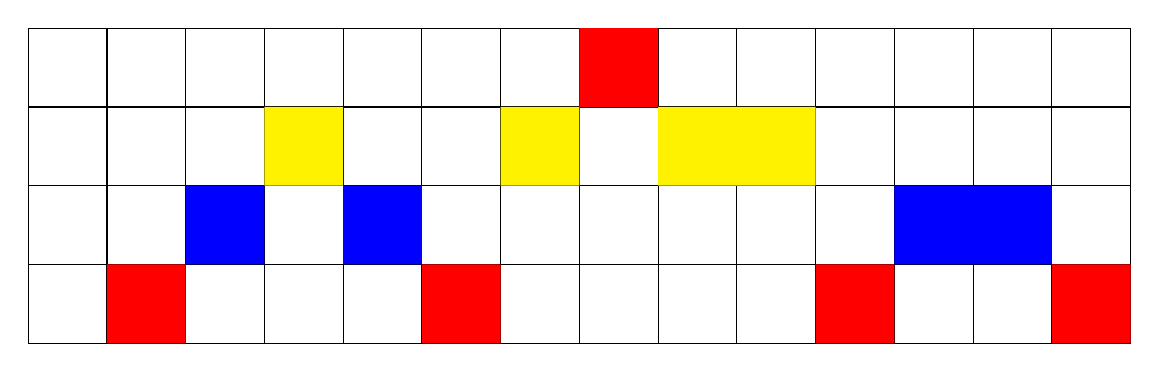
\begin{tikzpicture}
        \newcommand\fillGrid[2]{\fill[fill=#1,shift={#2}] (0,0) -- (0,1) -- (1,1) -- (1,0) --(0,0)}
        \draw[step=1cm](0,0) grid (14,4);
        \fillGrid{red}{(1,0)};
        \fillGrid{blue}{(2,1)};
        \fillGrid{yellow}{(3,2)};
        \fillGrid{blue}{(4,1)};
        \fillGrid{red}{(5,0)};
        \fillGrid{yellow}{(6,2)};
        \fillGrid{red}{(7,3)};
        \fillGrid{yellow}{(8,2)};
        \fillGrid{yellow}{(9,2)};
        \fillGrid{red}{(10,0)};
        \fillGrid{blue}{(11,1)};
        \fillGrid{blue}{(12,1)};
        \fillGrid{red}{(13,0)};
        \end{tikzpicture}
        \caption{任务先后关系。{\color{blue}蓝色}方格代表\textit{任务一},
            {\color{yellow}黄色}是 \textit{任务零},
            {\color{t2C}红色}是 \textit{任务二}}
        \label{fig:pi-1}
    \end{figure}

    这3个应用任务因为要竞争同一互斥资源mutex而相互制约。
    其中,任务TASK0的原始优先级最低,任务TASK1的原始优先级中等,任务TASK2的原始优先级最高。
    在使用mutex时采用优先级继承策略,并指定各任务在使用mutex时的PIP(优先级继承优先级)为8。
    
    \subsubsection{系统的运行流程}
    
    TaskStart任务挂起后,操作系统调度它所创建的3个应用任务,整个系统的运行流程如下:
    \begin{enumerate}
        \item TASK2拥有最高优先级10,最先开始运行,它在$t_1$时刻,执行\lstinline|OSMutexPend(mutex, 0, &err)|,
            成功获得互斥信号量mutex;
        \item $t_2$时刻,TASK2执行延时函数\lstinline|OSTimeDlyHMSM(0, 0, 0, 200)|被挂起200ms,
            操作系统调度优先级次之的TASK1运行;
        \item $t_3$时刻,TASK1执行 \lstinline|OSMutexPend(mutex, 0, &err)|申请互斥信号量失败后被阻塞,
            操作系统调度优先级最低的TASK0运行。TASK0执行\lstinline|OSMutexPend(mutex, 0, &err)|
            申请互斥信号量失败后也被阻塞。在TASK1和TASK0被阻塞的时候,由于当前拥有mutex的TASK2优先级最高,
            因此保持其优先级不变。当所有的应用任务都阻塞时,系统有一个空闲任务在运行,
            这个空闲任务是在初始化操作系统的时候创建的,它的优先级最低;
        \item $t_4$ 时刻,TASK2延时到并运行,它执行 \lstinline|OSMutexPost(mutex)|释放互斥信号量并由TASK1获得此信号量。
        \item $t_5$时刻TASK2将自己延时一段时间(150ms),任务回到运行状态;
        \item $t_6$ TASK1执行延时函数 \lstinline|OSTimeDlyHMSM(0, 0, 0, 200)| 后被挂起200ms,
        空闲任务运行;在$t_6$时刻TASK2因延时时间到恢复执行,它执行\lstinline|OSMutexPend(mutex, 0, &err)|
        申请互斥信号量失败后被阻塞,空闲任务运行。此时操作系统发现当前拥有信号量的任务TASK1的优先级低于TASK2的,
        因此将TASK1的优先级提升到PIP,但TASK1此时仍处于延时状态未运行;
        \item $t_7$时刻,TASK1延时到,它在高优先级(PIP)下继续运行,调用\lstinline|OSMutexPost(mutex)|
        释放互斥信号量并由TASK2获得此信号量,TASK1的优先级恢复到原来的高度,
        而TASK2因优先级较高而抢占TASK1运行(在t8时刻);
        \item TASK2又将自己延时一段时间(200ms),任务TASK1恢复执行后也将自己延时一段时间(300ms),空闲任务运行;t9时刻TASK2延时时间先到,它执行\lstinline|OSMutexPost(mutex)|释放互斥信号量,此时TASK0获得此信号量;
        \item $t_{10}$时刻,TASK2延时(150ms),任务TASK0被调度运行;TASK0在打印输出信息后,
        将自己延时(200ms),空闲任务运行;
        \item $t_{11}$ 时刻,TASK1延时到恢复运行。TASK1执行\lstinline|OSMutexPend(mutex, 0, &err)|
        申请互斥信号量失败后被阻塞;此时操作系统发现当前拥有信号量的TASK0优先级低于TASK1的,
        因此提升TASK0的优先级到PIP,空闲任务运行;
        \item $t_{12}$时刻,TASK2延时到恢复运行,它执行\lstinline|OSMutexPend(mutex, 0, &err)|
        申请互斥信号量失败后被阻塞;此时拥有信号量的TASK0的优先级已经被提升到了PIP,且高于TASK2的优先级,操作系统就没有针对TASK0再做优先级提升的工作。之后空闲任务运行;
        \item $t_{13}$时刻,TASK0延时到,在高优先级(PIP)下继续运行,它执行\lstinline|OSMutexPost(mutex)|
        释放互斥信号量,其优先级恢复到原来的高度,并由TASK2获得此信号量,TASK2抢占TASK0运行;
    \end{enumerate}
    
    \subsubsection{源程序说明}
    
    和实验二差不多,只是在低优先级占有资源是,会提升任务优先级。
    其中每个任务的代码如下。
    \begin{lstlisting}
void  Task (void *pdata) {
    INT8U  err;
    INT8U  id;
    id=*(int *)pdata;
    while(1) {
        kprint("task %b try to get the mutex.", id);
        // Acquire mutex to get continue
        OSMutexPend(mutex, 0, &err);
        kprint("task %b is getting the mutex.", id);
        // Wait 200 minisecond 
        OSTimeDlyHMSM(0, 0, 0, 200);
        kprint("task %b   releases the mutex.", id);
        // elease mutex
        OSMutexPost(mutex); 
        // Wait (3-id)*150 minisecond
        OSTimeDlyHMSM(0, 0, 0, (3-id)*150);
    }
}
    \end{lstlisting}

    \subsection{运行结果}
    
    和之前实验类似,编译并运行代码会得到如下输出。
    \begin{lstlisting}[language={}]
0000000000000000: uC/OS-II loaded
0400000000000000:
0600000000000000: task 01 try to get the mutex.
0B00000000000000: task 01 is getting the mutex.
1100000000000000: task 00 try to get the mutex.
4400000000000000: task 01   releases the mutex.
4900000000000000: task 00 is getting the mutex.
7E00000000000000: task 00   releases the mutex.
9800000000000000: task 01 try to get the mutex.
9E00000000000000: task 01 is getting the mutex.
D200000000000000: task 01   releases the mutex.
FA00000000000000: task 00 try to get the mutex.
FF00000000000000: task 00 is getting the mutex.
2601000000000000: task 01 try to get the mutex.
3701000000000000: task 00   releases the mutex.
3C01000000000000: task 01 is getting the mutex.
7101000000000000: task 01   releases the mutex.
B101000000000000: task 00 try to get the mutex.
B601000000000000: task 00 is getting the mutex.
C501000000000000: task 01 try to get the mutex.
EE01000000000000: task 00   releases the mutex.
F301000000000000: task 01 is getting the mutex.
2802000000000000: task 01   releases the mutex.
    \end{lstlisting}
    
    \section{哲学家就餐问题的实现}
    
    \subsection{实验目的}
    
    掌握在基于嵌入式实时操作系统µC/OS-II的应用中,任务使用信号量的一般原理。通过经典的哲学家就餐实验,了解如何利用信号量来对共享资源进行互斥访问。
    
    \subsection{原理及程序结构}
    
    \subsubsection{实验设计}
    
    五个哲学家任务(ph1、ph2、ph3、ph4、ph5)主要有两种过程:思考(即睡眠一段时间)和就餐。
    每个哲学家任务在就餐前必须申请并获得一左一右两支筷子,就餐完毕后释放这两支筷子。
    五个哲学家围成一圈,每两人之间有一支筷子。一共有五支筷子,在该实验中用了五个互斥信号量来代表。
    如图 \ref{fig:pe-1} 所示。
    \begin{figure}
     \centering
     \includegraphics[width=0.7\linewidth]{pe-1}
     \caption{哲学家就餐问题}
     \label{fig:pe-1}
    \end{figure}

    \subsection{源程序说明}
    
    任务的核心函数如下所示。
    \begin{lstlisting}
void  Task (void *pdata) {
    INT8U  err;
    INT8U  i;
    INT8U  j;
    
    i=*(int *)pdata;
    j=(i+1) % 5;
    
    while(1) {
        TASK_Thinking_To_Hungry(i);
        OSSemPend(fork[i], 0, &err);
        OSSemPend(fork[j], 0, &err);
        TASK_Eat(i);
        OSSemPost(fork[j]);
        OSSemPost(fork[i]);
        OSTimeDly(200);
    }
}
    \end{lstlisting}
    
    \lstinline|TASK_Thinkg_To_Hungry()| 与 \lstinline|TASK_Eat()| 为有关输出函数。其中包括输出和延时。
    
    \subsection{运行结果}
    
    和之前的实验一样,编译并运行的结果如下所示。
    \begin{lstlisting}[language={}]
0000000000000000: Ucos-II loaded
0400000000000000:
0600000000000000: Philosopher 01 is thinking.
0B00000000000000:
0D00000000000000: Philosopher 02 is thinking.
1200000000000000:
1500000000000000: Philosopher 03 is thinking.
1A00000000000000:
1C00000000000000: Philosopher 04 is thinking.
2100000000000000:
2300000000000000: Philosopher 05 is thinking.
2900000000000000:
3700000000000000: Philosopher 05 is hungry.
3C00000000000000:
4400000000000000: Philosopher 04 is hungry.
4900000000000000:
5100000000000000: Philosopher 03 is hungry.
5600000000000000:
5900000000000000: Philosopher 05 is eating.
5E00000000000000:
6500000000000000: Philosopher 02 is hungry.
6A00000000000000:
7300000000000000: Philosopher 01 is hungry.
7800000000000000:
7A00000000000000: Philosopher 04 is eating.
8000000000000000:
8E00000000000000: Philosopher 03 is eating.
9300000000000000:
A100000000000000: Philosopher 05 is thinking.
A600000000000000:
A900000000000000: Philosopher 02 is eating.
AE00000000000000:
BC00000000000000: Philosopher 04 is thinking.
C100000000000000:
C300000000000000: Philosopher 01 is eating.
C900000000000000:
CB00000000000000: Philosopher 05 is hungry.
D000000000000000:
DE00000000000000: Philosopher 03 is thinking.
E300000000000000:
E600000000000000: Philosopher 05 is eating.
EB00000000000000:
F300000000000000: Philosopher 04 is hungry.
F800000000000000:
0001000000000000: Philosopher 02 is thinking.
0501000000000000:
1301000000000000: Philosopher 01 is thinking.
1801000000000000:
1A01000000000000: Philosopher 03 is hungry.
2001000000000000:
2201000000000000: Philosopher 04 is eating.
2701000000000000:
3501000000000000: Philosopher 05 is thinking.
3A01000000000000:
4201000000000000: Philosopher 02 is hungry.
4701000000000000:
5001000000000000: Philosopher 03 is eating.
5501000000000000:
    \end{lstlisting}
    
    
    \section{其余实验输出结果}
    
    \subsection{消息队列}
    \begin{lstlisting}[language={}]
0000000000000000: uC/OS-II loaded
0400000000000000:
0600000000000000: Add message to queue1
0A00000000000000: the queue1 00 add message0
3300000000000000: the queue1 01 add message1
5C00000000000000: the queue1 02 add message2
8500000000000000: the queue1 03 add message3
AE00000000000000: the queue1 04 add message4
D700000000000000: the queue1 05 add message5
0001000000000000: Add message to queue2
0401000000000000: the queue2 00 add messageA
2C01000000000000: the queue2 01 add messageB
5501000000000000: the queue2 02 add messageC
7E01000000000000: the queue2 03 add messageD
A701000000000000: the queue2 04 add messageE
D001000000000000: the queue2 05 add messageF
F901000000000000: Clear up the queue2
FD01000000000000: the queue2'information
0202000000000000: NextMsg:,  NumMsg:00000000,  QSize:06000000.
2402000000000000: Task 00 has got the message5
2902000000000000: Task 01 has got the message4
8802000000000000: Not successful delete queue2
8D02000000000000: Add message to queue1
9202000000000000: the queue1 00 add message0
BB02000000000000: the queue1 01 add message1
E302000000000000: the queue1 is full, don't add.
0C03000000000000: the queue1 is full, don't add.
3503000000000000: the queue1 is full, don't add.
5E03000000000000: the queue1 is full, don't add.
8703000000000000: Add message to queue2
8B03000000000000: Task 04 has got the messageA.
9103000000000000:
9303000000000000: the queue2 00 add messageA
BC03000000000000: the queue2 01 add messageB
E503000000000000: the queue2 02 add messageC
0E04000000000000: the queue2 03 add messageD
3704000000000000: the queue2 04 add messageE
6004000000000000: the queue2 05 add messageF
8904000000000000: the queue2'information
8D04000000000000: NextMsg:messageB,  NumMsg:05000000,  QSize:06000000.
E504000000000000: Task 01 has got the message1
1005000000000000: Not successful delete queue2
1605000000000000: Add message to queue1
1A05000000000000: the queue1 00 add message0
2305000000000000: Task 00 has got the message0
4705000000000000: the queue1 01 add message1
7005000000000000: the queue1 is full, don't add.
9805000000000000: the queue1 is full, don't add.
C105000000000000: the queue1 is full, don't add.
EA05000000000000: the queue1 is full, don't add.
1306000000000000: Add message to queue2
1806000000000000: the queue2 00 add messageA
4006000000000000: the queue2 is full, don't add.
5206000000000000: Task 04 has got the messageB.
5706000000000000:
6F06000000000000: the queue2 02 add messageC
9806000000000000: the queue2 is full, don't add.
C006000000000000: the queue2 is full, don't add.
E906000000000000: the queue2 is full, don't add.
1207000000000000: Clear up the queue2
1607000000000000: the queue2'information
1B07000000000000: NextMsg:,  NumMsg:00000000,  QSize:06000000.
9A07000000000000: Not successful delete queue2
9F07000000000000: Add message to queue1
A407000000000000: the queue1 is full, don't add.
B107000000000000: Task 01 has got the message1
D007000000000000: the queue1 01 add message1
F907000000000000: the queue1 is full, don't add.
1B08000000000000: Task 00 has got the message1
2608000000000000: the queue1 03 add message3
4F08000000000000: the queue1 is full, don't add.
7808000000000000: the queue1 is full, don't add.
A108000000000000: Add message to queue2
A508000000000000: the queue2 00 add messageA
CD08000000000000: the queue2 01 add messageB
F608000000000000: the queue2 02 add messageC
1609000000000000: Task 04 has got the messageA.
1C09000000000000:
2509000000000000: the queue2 03 add messageD
4E09000000000000: the queue2 04 add messageE
7709000000000000: the queue2 05 add messageF
A009000000000000: the queue2'information
A409000000000000: NextMsg:messageB,  NumMsg:05000000,  QSize:06000000.
240A000000000000: Already successful delete queue2
2A0A000000000000: Add message to queue1
2E0A000000000000: the queue1 is full, don't add.
580A000000000000: the queue1 is full, don't add.
750A000000000000: Task 01 has got the message3
840A000000000000: the queue1 02 add message2
AD0A000000000000: the queue1 is full, don't add.
D60A000000000000: the queue1 is full, don't add.
FF0A000000000000: the queue1 is full, don't add.
160B000000000000: Task 00 has got the message2
2B0B000000000000: Add message to queue2
300B000000000000: Clear up the queue2
AC0B000000000000: Add message to queue1
B10B000000000000: the queue1 00 add message0
D50B000000000000: queue2  is empty,04 can't got the message.
DE0B000000000000: the queue1 is full, don't add.
    \end{lstlisting}
    \subsection{时钟中断}
    \begin{lstlisting}[language={}]
0000000000000000: uC/OS-II loaded
0400000000000000:
0600000000000000: Task2 is try to get semaphore.
0B00000000000000: Task2 has Succeed to obtain semaphore.
1200000000000000: Task2 is delayed.
1600000000000000: Task3 has got the CPU
8D00000000000000: Task1 is try to get semaphore.
9600000000000000: Task3 has got the CPU
1201000000000000: Task3 has got the CPU
8E01000000000000: Task3 has got the CPU
0A02000000000000: Task3 has got the CPU
8002000000000000: The delay of Task2 finished .
8502000000000000: Task2 release semaphore.
8A02000000000000: Task1 has Succeed to obtain semaphore.
9002000000000000: Task1 is delayed.
9502000000000000: Task3 has got the CPU
1103000000000000: Task3 has got the CPU
8903000000000000: The delay of Task1 finished .
8F03000000000000: Task1 release semaphore.
9403000000000000: Task2 is try to get semaphore.
9903000000000000: Task2 has Succeed to obtain semaphore.
9F03000000000000: Task2 is delayed.
A403000000000000: Task3 has got the CPU
2004000000000000: Task3 has got the CPU

    \end{lstlisting}
    \subsection{内存管理}
    \begin{lstlisting}[language={}]
0000000000000000: uC/OS-II loaded
0400000000000000:
0600000000000000:
0800000000000000: The pointer to the begining of memory address is: 44000020
1100000000000000: the size of blocks in this memory area is: 80000000
1900000000000000: the number of free blocks in this memory area is: 02000000
2100000000000000: the number of using blocks in this memory area is: 00000000
2A00000000000000:
6800000000000000: First memory application HAS accept.
6E00000000000000:
7000000000000000: The pointer to the begining of memory address is: 44000020
7900000000000000: the size of blocks in this memory area is: 80000000
8100000000000000: the number of free blocks in this memory area is: 01000000
8900000000000000: the number of using blocks in this memory area is: 01000000
9200000000000000:
D000000000000000: Second memory application HAS accept.
D700000000000000:
D900000000000000: The pointer to the begining of memory address is: 44000020
E100000000000000: the size of blocks in this memory area is: 80000000
E900000000000000: the number of free blocks in this memory area is: 00000000
F200000000000000: the number of using blocks in this memory area is: 02000000
FB00000000000000:
3901000000000000: Third memory alpplication NOT accept.
3F01000000000000:
4101000000000000:
4301000000000000: The pointer to the begining of memory address is: 44000020
4C01000000000000: the size of blocks in this memory area is: 80000000
5401000000000000: the number of free blocks in this memory area is: 00000000
5C01000000000000: the number of using blocks in this memory area is: 02000000
6501000000000000:
A301000000000000: Third memory didn't exist.
A801000000000000:
AB01000000000000: The pointer to the begining of memory address is: 44000020
B301000000000000: the size of blocks in this memory area is: 80000000
BB01000000000000: the number of free blocks in this memory area is: 00000000
C401000000000000: the number of using blocks in this memory area is: 02000000
CC01000000000000:
0002000000000000: Second memory has been released.
0502000000000000:
0802000000000000: The pointer to the begining of memory address is: 44000020
1002000000000000: the size of blocks in this memory area is: 80000000
1802000000000000: the number of free blocks in this memory area is: 01000000
2102000000000000: the number of using blocks in this memory area is: 01000000
2902000000000000:
5D02000000000000: First memory has been released.
6202000000000000:
6502000000000000: The pointer to the begining of memory address is: 44000020
6D02000000000000: the size of blocks in this memory area is: 80000000
7502000000000000: the number of free blocks in this memory area is: 02000000
7E02000000000000: the number of using blocks in this memory area is: 00000000
8602000000000000:
    \end{lstlisting}
\end{document}